\documentclass[12pt]{article}   	% use "amsart" instead of "article" for AMSLaTeX format
\usepackage[margin=1in]{geometry}                		% See geometry.pdf to learn the layout options. There are lots.
\geometry{letterpaper}                   		% ... or a4paper or a5paper or ... 
%\geometry{landscape}                		% Activate for for rotated page geometry
\usepackage[parfill]{parskip}    		% Activate to begin paragraphs with an empty line rather than an indent
\usepackage{graphicx}				% Use pdf, png, jpg, or eps� with pdflatex; use eps in DVI mode
								% TeX will automatically convert eps --> pdf in pdflatex	
\usepackage{amsmath}
\usepackage{amssymb}
\usepackage{amsthm}
\usepackage{mathrsfs}
\usepackage{amsbsy}
\usepackage{braket}
\usepackage{enumitem}
\usepackage{listings}
\usepackage{dsfont}
\usepackage{hyperref}
\hypersetup{colorlinks=true, urlcolor=cyan}
\usepackage [english]{babel}
\usepackage [autostyle, english = american]{csquotes}
\MakeOuterQuote{"}


\title{Trochoidal Colloidal Swimmers \\ \large Computational Final Project}
\author{Paul McNulty}
\date{12/16/2016}							% Activate to display a given date or no date

\begin{document}
\maketitle

\begin{abstract}
It has been demonstrated that a particular colloidal particle comprised primarily of a dielectric sphere with a small metallic cube embedded in its surface traces out interesting and complex rosette-like patterns when subjected to a non-uniform light field. This motion is described by a set of coupled stochastic differential equations, which are derived given reasonable assumptions about the colloid's interaction with the light field. In this paper, we explore how the motion changes if we account for forces that were assumed to be negligible in the original analysis. To do this, we first suppose the inertial term in the force equation is non-negligible, and second we suppose the radiation pressure has a non-negligible affect on the translational velocity. Included in this paper is a description of the Euler-Maruyama method for integrating stochastic differential equations.
\end{abstract} 

\section*{Trochoidal Colloids}
The basis for this paper is laid out in "Trochoidal Trajectories of Self-Propelled Janus Particles in a Diverging Laser Beam" by H. Moyses, J. Palacci, S. Sacanna, and D. Grier [1]. Typically, active particles exhibit ballistic and brownian motion. The motion of the particles studied here resembles rosette curves known as trochoids. The schematic of the particle and a trace of its motion can be seen in \textbf{Figure 1}. The particles are comprised of a metallic hematite cube which is embedded in a transparent dielectric sphere of 3-methacryloxypropyl trimethoxysilane (TPM), the radius of which is $a=1.0\mu m$. The particles are placed in a water solution and sediment to the bottom glass surface with the orientation shown in \textbf{Figure 1}. The cube remains in contact with the glass throughout the trajectory. The motion is driven by the diverging laser beam focused a distance $L=10.0 \mu m$ below the glass as shown in \textbf{Figure 1}. The light heats the hematite cube, producing a temperature gradient around the particle which creates a local flow field. This propels the particle in the direction opposite the cube. Furthermore, because the light has a negligible interaction with the rest of the particle as compared to the cube, the radiation pressure produces a torque on the particle, causing it to rotate and giving rise to the looping motion seen. The intensity of the light field points radially outward and has the form of a gaussian 

\begin{equation}
\vec{I}(r) = I_0 exp(-\frac{r^2}{2\sigma^2}).
\end{equation}
The rotation due to the radiation pressure is given by
\begin{equation}
\omega(r) = \mu_{\theta} \alpha_r \frac{a}{\sqrt{2}}I(r) \frac{r}{\sqrt{r^2 + L^2}} \hat{r} \times \hat{n} ,
\end{equation}
and since the radiation pressure has a negligible affect on the translational velocity, it can be modeled as
\begin{equation}
v(r) \approx \frac{v_0}{I_0}I(r).
\end{equation} 
Thus the equations of motion are given by the stochastic differential equations
\begin{equation}
\dot{x}(t) = v(r(t))\cos(\phi(t)) + \zeta(t)
\end{equation}
\begin{equation}
\dot{y}(t) = v(r(t))\sin(\phi(t)) + \zeta(t)
\end{equation}
\begin{equation}
\dot{\phi}(t) = \frac{x(t) \dot{y}(t) - y(t)\dot{x}(t)}{d \sqrt{r^2(t) + L^2}} + \sqrt{\frac{3}{4a^2}}\zeta(t) .
\end{equation}

The term $\zeta(t)$ is the stochastic noise term and is characterized by thermal fluctuations. These equations can be integrated via the Euler-Maruyama method, and yield a picture qualitatively similar to the motion traced out by the particles in the laboratory. However, due to the random nature of the $\zeta$ term, I found the variability from one run to another to be quite large. 

\begin{center}
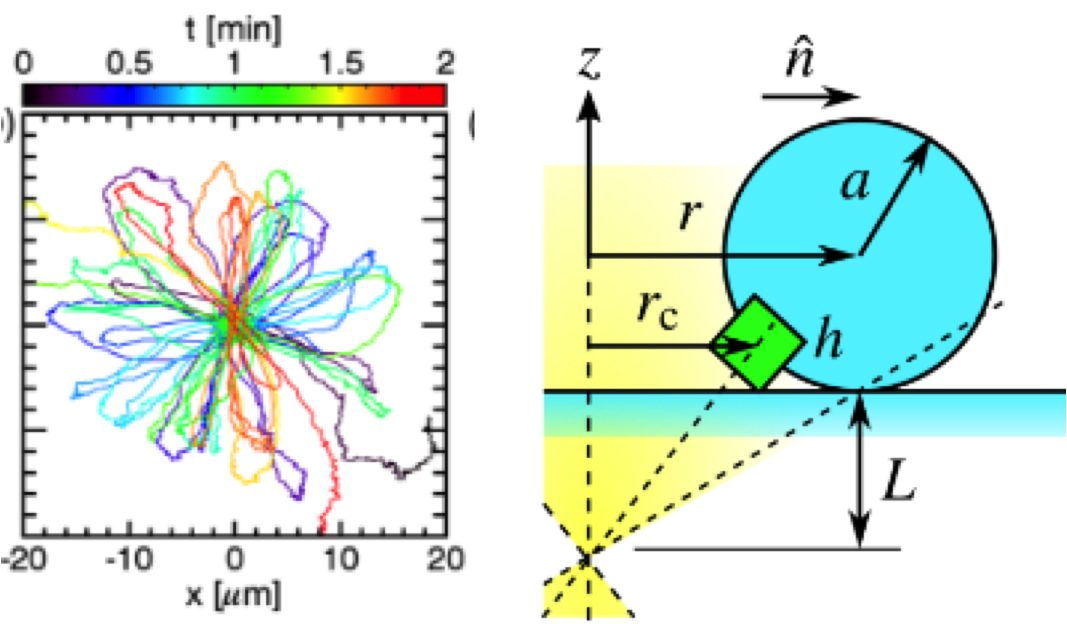
\includegraphics[scale = 0.5]{fig1.png}
\\
\textbf{Figure 1}: Shown at left is the traced motion of these colloidal particles. At right is a schematic of the particle, giving the orientation of the cube and the $\hat{n}$ vector. For this setup, the radius $a = 1.0 \mu m$ and the laser was focused at $L = 10.0 \mu m$. Both images were taken from H. Moyses et al.
\end{center}

\section*{Euler-Maruyama Scheme}
In "Numerical Solution of Stochastic Differential Equations in Finance", T. Sauer details the Euler-Maruyama scheme for integrating stochastic differential equations. Given a differential equation of the form (known as the Langevin equation)
\begin{equation}
dX(t) = -\mu X(t)dt + \sigma dW_t
\end{equation}
where $dW_t$ is the Brownian noise, the numerical solution is given by
\begin{equation}
y_0 = X_0
\end{equation}
\begin{equation}
y_{i+1} = y_i - \mu y_i \Delta t_i + \sigma \Delta W_i .
\end{equation}
Without the Brownian noise term, this simply reduces to Forward Euler. For our problem, the Brownian term $\zeta(t)$ can be modeled appropriately by drawing random numbers from a normally distributed gaussian scaled by the square root of the product of the diffusion coefficient $D = \frac{k_b T}{6\pi \nu a}$, where $k_b$ is the Boltzmann constant, $T$ is the tempurature, $\nu$ is the viscosity, and $a$ is the radius, and the time step $\Delta t$. Since we have a system of coupled equations, a different $\zeta(t)$ needs to be generated for each dimension at each time-step. Because this method is sort of a messy Forward Euler, the error scales as $\mathcal{O}(N/2)$ for the number of steps $N$. To check that this method was working properly, I ran it with and without noise and ensured it qualitatively matched the plots generated in H. Moyses et al.'s paper. These plots can be seen in \textbf{Figure 2}.

\begin{center}
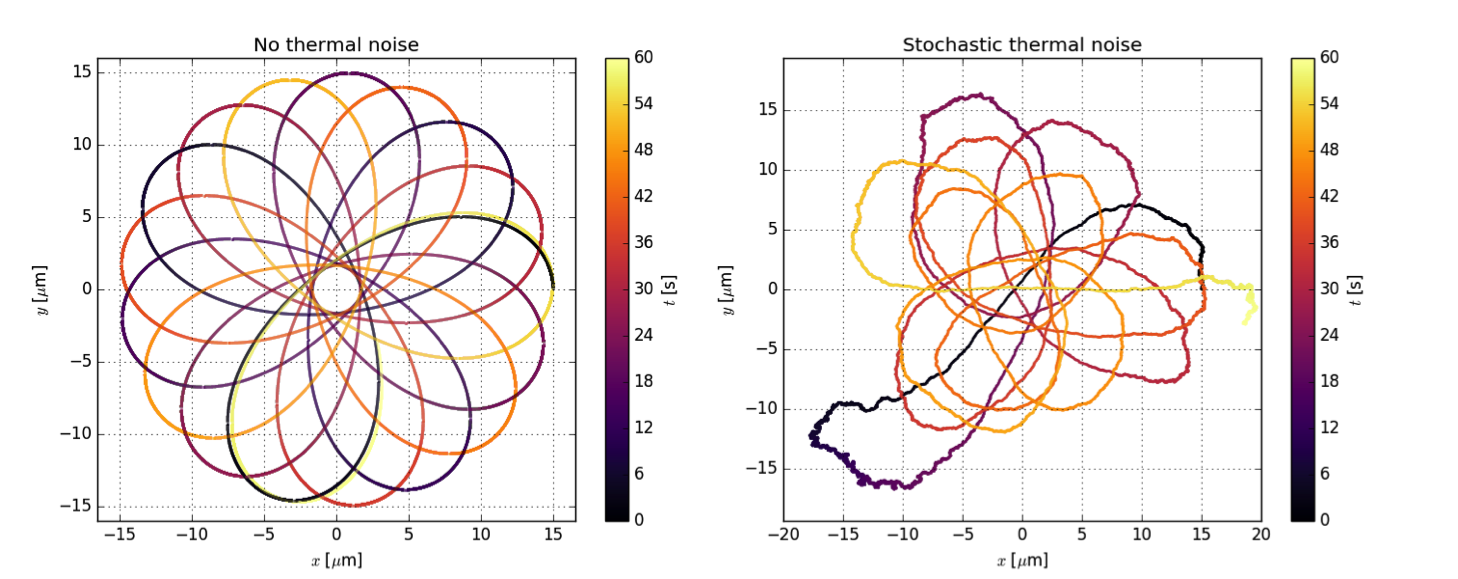
\includegraphics[scale = 0.5]{fig2.png}
\\
\textbf{Figure 2}: At left is the result of integrating equations (4), (5), and (6) neglecting $\zeta(t)$. This shows that qualitatively the equations of motion match the observed behavior. Plotted at right is the result of turning the Brownian noise term on for room temperature at $T=294K$.
\end{center}

\section*{Incorporating Inertia}
To move beyond the work done in the paper, I attempted to incorporate a mass term in the translational equations of motion. In many of these colloidal problems, the inertia term is negligible and so can be ignored, but it could be interesting to see if any details about how the motion would change if the mass term became important. To do this, I started with the equation
\begin{equation}
m\ddot{\vec{r}} +\gamma \dot{\vec{x}} = \vec{v} + \zeta(t),
\end{equation}
where $\vec{v}$ is comprised of $v_x = v(r(t))\cos(\phi(t))$ and $v_y = v(r(t))\sin(\phi(t))$ and $\gamma$ is a drag coefficient. This led to the system of differential equations
\begin{equation}
\dot{\vec{u}} = \frac{\gamma}{m}(\vec{v} - \vec{u}) + \zeta(t)
\end{equation}
\begin{equation}
\dot{\vec{x}} = \vec{u} 
\end{equation}
which were again solved via the Euler-Maruyama scheme. The noise term should now scale with mass in some way, but here for simplicity it was taken to still scale as $\sqrt{D\Delta t}$. To see how these new equations of motion changed for non-negligible mass, I integrated equations (11), (12), and (6) with and without the noise term for a variety of values of the ratio $\frac{\gamma}{m}$, of which exemplary plots can be seen in \textbf{Figure 3}. Without the noise term, the non-negligible mass causes the motion to break the trochoidal pattern and become circular. The motion with the noise is more difficult to analyze, but it does appear to  have less eccentric loops at later times. For high mass, the motion starts out ballistic until it gets to some characteristic distance such that the light intensity drops off and the particle begins moving very slowly. At this point, the thermal fluctuations are dominant and the particle seemingly undergoes a random walk.

\begin{center}
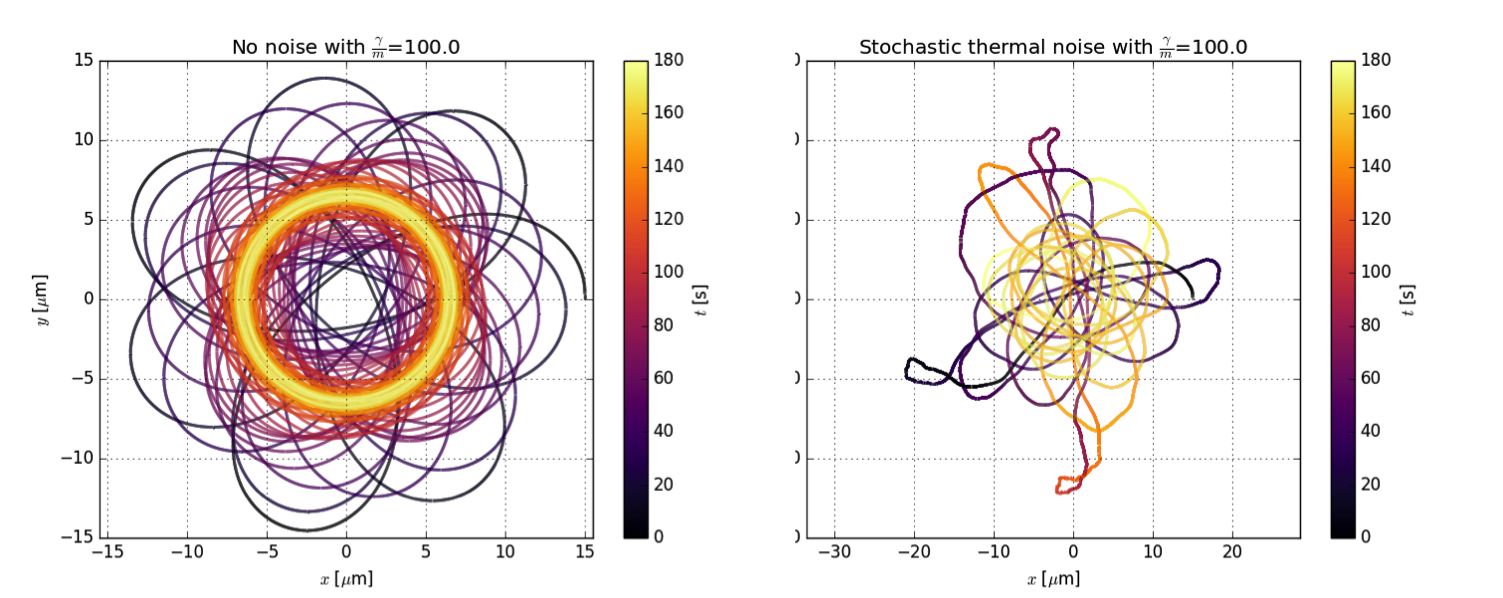
\includegraphics[scale = 0.5]{fig3.png}
\\
\textbf{Figure 3}: At left is the result of integrating equations (11), (12), and (6) neglecting the noise terms for the ratio $\frac{\gamma}{m} = 100.0$. Note how the loops are damped and the particle eventually settles into a circular trajectory. Plotted at right is the result with the Brownian terms on, indicating again that the motion is eventually damped into smaller loops.
\end{center}

\section*{Adding Radiation Pressure}
Another interesting prospect is to consider a particle constructed such that the light interacts with more than the small cube. In the paper it is demonstrated that there is a small difference on average between the particle's velocity when moving towards the center versus moving away, with the former being slower than the later. This indicates that the radiation pressure is having some affect on the particles translational velocity, albeit not enough to be incorporated in equations (4) and (5). To incorporate this radiation pressure, the equations of motion change to 
\begin{equation}
\dot{x} = v(r(t))\cos(\phi(t)) + \frac{\pi a^2}{\beta} I(r)\cos{(\arctan{(y/x)})} +  \zeta(t)
\end{equation}
\begin{equation}
\dot{y} = v(r(t))\sin(\phi(t)) + \frac{\pi a^2}{\beta} I(r)\sin{(\arctan{(y/x)})} +  \zeta(t).
\end{equation}
Because the radiation pressure is what cause the rotations, equation (6) remains unchanged. For un-perturbed motion with increasing radiation pressure, I expected to find a characteristic intensity such that the particle would be deflected completely from the center, creating much tighter outer-loops as the particle traversed the light field. However, as I varied the intensity and the particle was deflected from the center, the particle executed a motion that more resembled a fan. Despite this qualitative difference in the unperturbed motion, it is difficult to say if the motion with noise is significantly changed. Examples of the unperturbed and perturbed motion can be seen in \textbf{Figure 4}. Unsurprisingly, for very high intensity the particle is ejected from the influence of the light field almost immediately. The effects of intensity on the motion could be an interesting avenue for further studies. 

\begin{center}
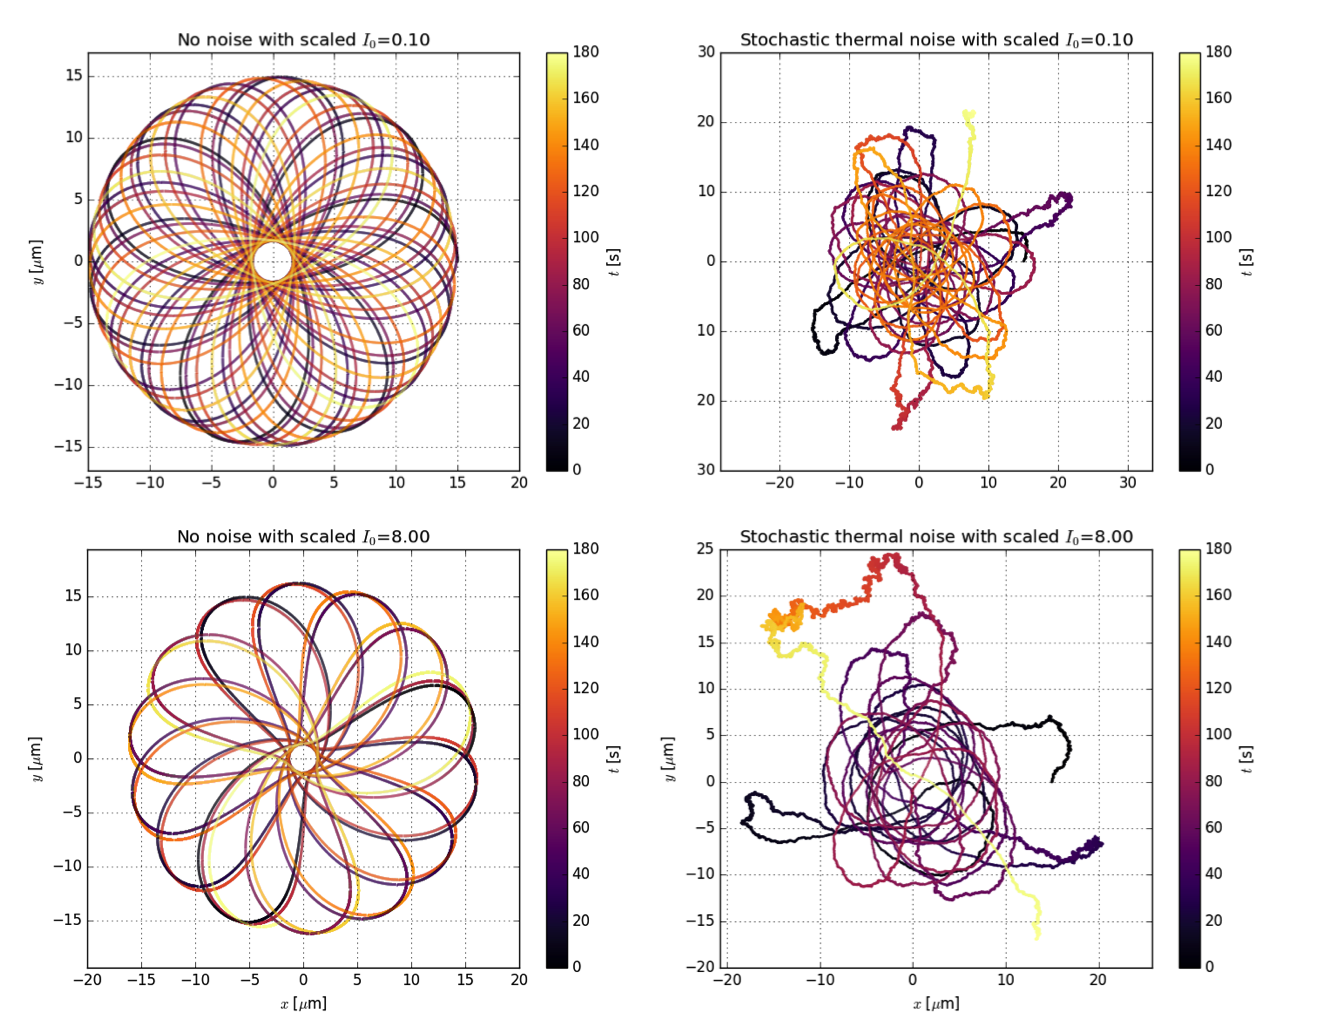
\includegraphics[scale = 0.5]{fig4.png}
\\
\textbf{Figure 4}: The left most plots are the result of integrating equations (6), (13), and (14) with low (top) and high (bottom) intensity while neglecting the noise terms. From the bottom left plot it is evident that the particle is being deflected away from the center, causing a fan-like trajectory. However, when comparing the plots at right it is difficult to say if there is any qualitative difference in the motion.
\end{center}

\section*{References}
[1] H. Moyses, J. Palacci, S. Sacanna, D. G. Grier. June, 2016. "Trochoidal Trajectories of Self-Propelled Janus Particles in a Diverging Laser Beam" \textit{Soft Matter} \textbf{16}, 6357-6364 (2016).\\
\href{http://physics.nyu.edu/grierlab/swimdance9c/}{http://physics.nyu.edu/grierlab/swimdance9c/}
\\[0pt]
[2] T. Sauer, "Numerical Solution of Stochastic Differential Equations in Finance"\\
\href{http://math.gmu.edu/~tsauer/pre/sde.pdf}{http://math.gmu.edu/~tsauer/pre/sde.pdf}

\end{document}